% This is auto-generated file: do not edit!
% Exported from microMathematics Plus, version 2.17.2


Сейчас мы построим несколько
графиков функций в полярной
системе координат. Каждая точка в
этой системе определяется
расстоянием r от начала координат
и углом f относительно оси
абсцисс.
\begin{center}\begin{tabular}{c} 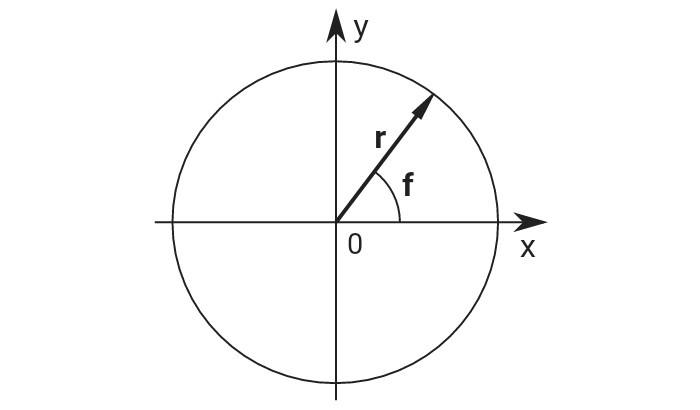
\includegraphics[resolution=320]{graphics/polar_plot_fig1.png} \end{tabular}\end{center}

Угловая координата f будет являться
нашей независимой переменной,
которую мы зададим в виде
интервала:
\begin{center}\begin{tabular}{c}
  $f := \left[ 0.01,\, 0.05 \,..\, 300 \right]$
\end{tabular}\end{center}

Расстояние от начала координат r -
это зависимая переменная. Каждую
пару значений f и r можно
пересчитать в декартовы координаты
x и y, используя следующие
формулы:
\begin{center}\begin{tabular}{cc}
  $x(r) := r \cdot cos \left( f\right) $ &
  $y(r) := r \cdot sin \left( f\right) $ \cr
\end{tabular}\end{center}

\subsection{Улитка}

Первую функцию будем определять в
три шага. На первом шаге введём
функцию, которая описывает простое
''колесо''. Эта функция зависит от
трёх коэффициентов A, B, q. Их
изменение позволяет значительно
менять вид получаемых кривых: 
\begin{center}\begin{tabular}{ccc}
  $A := 1.1$ &
  $B := 1.271$ &
  $q := 2$ \cr
\end{tabular}\end{center}
\begin{center}\begin{tabular}{c}
  $r1(f) := A + 2 \cdot {sin \left( B \cdot f\right) }^{q}$
\end{tabular}\end{center}

Далее добавим поле графика,
используя кнопку ''Вставить'' на
верхней панели инструментов или
кнопку ''Вставить график функции''
на нижней панели:
\begin{center}\begin{tabular}{c} 
\includegraphics[resolution=320]{graphics/polar_plot_fig2.png} \end{tabular}\end{center}

Однако вместо пары f и r мы должны
использовать в поле графика их
декартовы образы, которые
получаются, если взять приведённые
выше формулы преобразований и
подставить в них r1(f) в качестве
символьного аргумента:
\begin{center}\begin{tabular}{c} 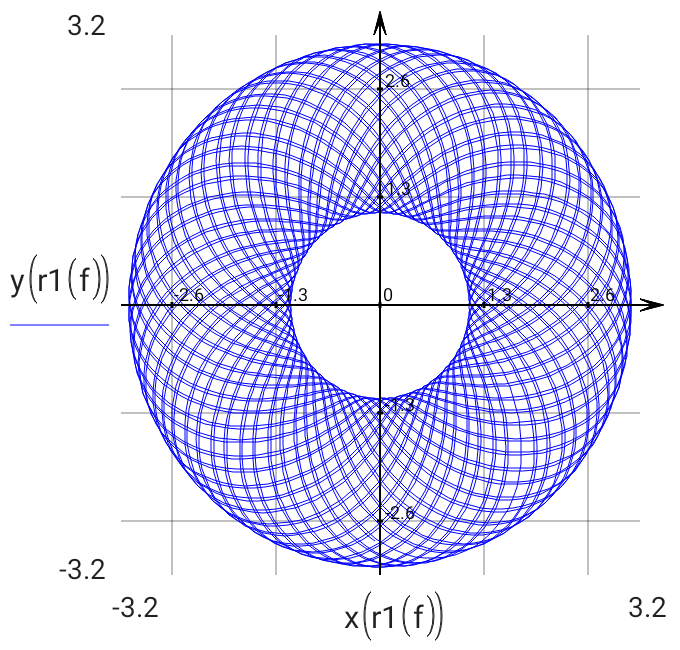
\includegraphics[resolution=320]{graphics/polar_plot_fig3.png} \end{tabular}\end{center}

Затем немного модифицируем наше
''колесо'':
\begin{center}\begin{tabular}{c}
  $r2(f) := A + 2 \cdot {sin \left( B \cdot f + 1 \cdot r1 \left( f\right) \right) }^{q}$
\end{tabular}\end{center}
\begin{center}\begin{tabular}{c} 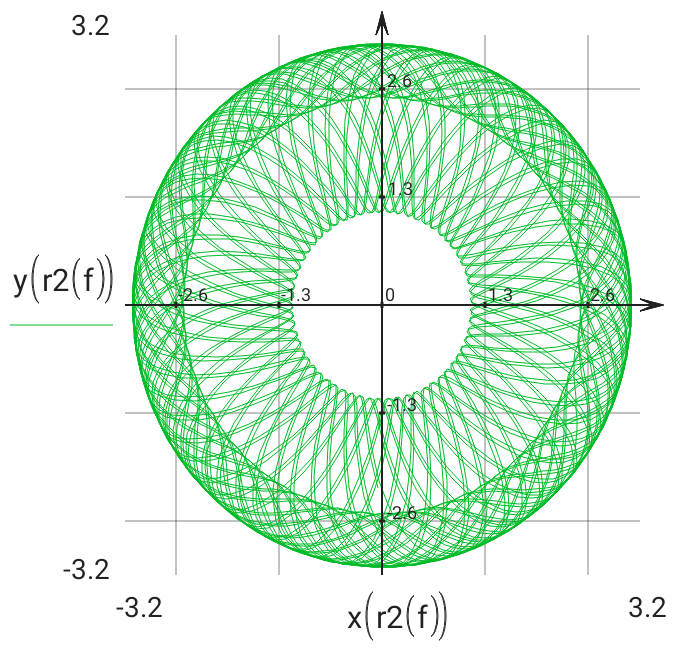
\includegraphics[resolution=320]{graphics/polar_plot_fig4.png} \end{tabular}\end{center}

Наконец, зададим итоговую функцию
скалированием функции r2(f),
используя при этом операцию
преобразования вещественного числа
в целое, которая выглядит как
ступенчатая функция. В итоге,
получилась вот такая замечательная
улитка:
\begin{center}\begin{tabular}{c}
  $r(f) := r2 \left( f\right)  \cdot floor \left( f\right)  / 10$
\end{tabular}\end{center}
\begin{center}\begin{tabular}{c} 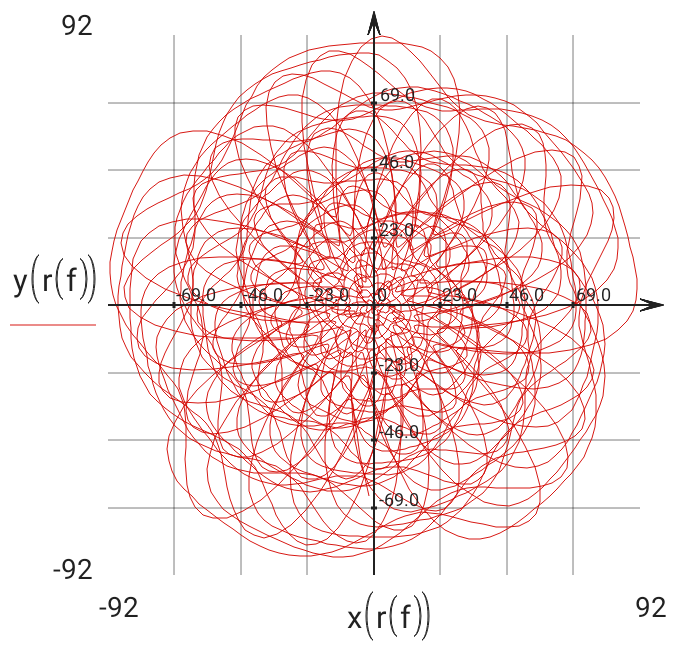
\includegraphics[resolution=320]{graphics/polar_plot_fig5.png} \end{tabular}\end{center}

\subsection{Японский клён}

Японский клён получил широкую
известность благодаря необычным
формам и окраске своих листьев.
Данный пример показывает, как
такой лист может быть описан
математически и нарисован как
кривая в полярной системе
координат:
\begin{center}\begin{tabular}{c}
  $f := \left[ 0.01,\, 0.02 \,..\, 100 \right]$
\end{tabular}\end{center}
\begin{center}\begin{tabular}{cc}
  $x(r) := r \cdot cos \left( f\right) $ &
  $y(r) := r \cdot sin \left( f\right) $ \cr
\end{tabular}\end{center}
\begin{center}\begin{tabular}{c}
  $s1(f) := \left( 1 + sin \left( f\right)  \right) \cdot \left( 1 - 0.9 \cdot  \left| sin \left( 4 \cdot f\right)  \right|  \right)$
\end{tabular}\end{center}
\begin{center}\begin{tabular}{c}
  $s2(f) := 0.9 + 0.05 \cdot cos \left( 200 \cdot f\right) $
\end{tabular}\end{center}
\begin{center}\begin{tabular}{c}
  $r(f) := floor \left( f\right)  \cdot s1 \left( f\right)  \cdot s2 \left( f\right)  + random \left( 2\right)  - 1$
\end{tabular}\end{center}
\begin{center}\begin{tabular}{c} 
\includegraphics[resolution=320]{graphics/polar_plot_fig6.png} \end{tabular}\end{center}

http://en.wikipedia.org/wiki/Acer\_palmatum